We need to optimize our process to be TTL compatible (5V logic levels) and at the same time being as fast and power efficient as possible.
In order to have a good propagation delay with a technology node of around $1\mu m$ we will have to have gates with up to four stacked MOS transistors.

Acceptable input signal voltages range from 0 volts to 0.8 volts for a low logic state, and 2 volts to 5 volts for a high logic state.
Acceptable output signal voltages shall range from 0 volts to 0.5 volts for a low logic state, and 2.7 volts to 5 volts for a high logic state\footnote{\url{https://www.allaboutcircuits.com/textbook/digital/chpt-3/logic-signal-voltage-levels}}

\begin{figure}[H]
	\centering
	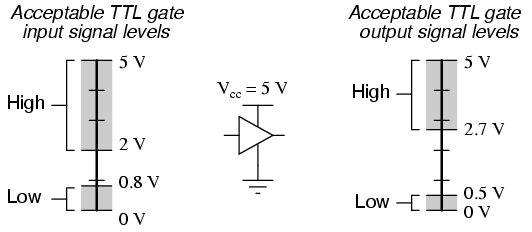
\includegraphics[scale=0.5]{logic_levels.png}
	\caption{TTL logic levels}
	\label{TTL_logic_levels}
\end{figure}

As shown in \autoref{TTL_logic_levels} we have some margin to make our PMOS and NMOS transistors work with each other in order to form a CMOS circuit which is actually working without getting warm.

Or more clearly defined
\begin{equation}
V_{off} \leq 0.8V
\end{equation}
and
\begin{equation}
V_{on} \geq 2V
\end{equation}
which are limits, elementary to our design.